%-------------------------------------------------------------------------------
%                      Template Naskah Skripsi Ilmu Komputer
%               	Berdasarkan format Teknik Informatika FMIPA UNNES
% 						(c) Aji Purwinarko 
%-------------------------------------------------------------------------------

%Template pembuatan skripsi.
\documentclass{skripsi}

% prefiks pada daftar gambar dan tabel
\usepackage[titles]{tocloft}
\renewcommand\cftfigpresnum{Gambar\  }
\renewcommand\cfttabpresnum{Tabel\   }

% hyperlink dan table of content
\usepackage[hidelinks]{hyperref}

\newlength{\mylenf}
\settowidth{\mylenf}{\cftfigpresnum}
\setlength{\cftfignumwidth}{\dimexpr\mylenf+2em}
\setlength{\cfttabnumwidth}{\dimexpr\mylenf+2em}

%Untuk Bold Face pada Keterangan Gambar
\usepackage[labelfont=bf]{caption}

%Untuk caption dan subcaption
\usepackage{caption}
\usepackage{subcaption}


\usepackage[utf8]{inputenc}
\usepackage[english]{babel}
\usepackage{enumitem}
\usepackage{apacite}
\usepackage{natbib}
\bibliographystyle{UNNESapa}
\AtBeginDocument{
	\renewcommand{\BBOP}{}
	\renewcommand{\BBCP}{}
}
\setcitestyle{authoryear, open={(},close={)},notesep={: }}

%\usepackage[none]{hyphenat}
% setting hyphenation pada paragraf
\tolerance=1
\emergencystretch=\maxdimen
\hyphenpenalty=10000
\hbadness=10000

%\newcommand\listappendixname{DAFTAR LAMPIRAN}
%\newcommand\appcaption[1]{%
%   \addcontentsline{app}{chapter}{#1}}
%\makeatletter
%\newcommand\listofappendices{%
%   \chapter*{\listappendixname}\@starttoc{app}}
%\makeatother

\newcommand{\listappendicesname}{DAFTAR LAMPIRAN}
\newlistof{appendices}{apc}{\listappendicesname}
\newcommand{\appendices}[1]{\addcontentsline{apc}{appendices}{#1}}
\newcommand{\newappendix}[1]{\section*{#1}\appendices{#1}}
%\makeatletter
%\renewcommand\section{\@startsection {section}{1}{\z@}%
%  {-3.5ex \@plus -1ex \@minus -.2ex}%
%  {2.3ex \@plus.2ex}%
%  {\centering\normalfont\Large\bfseries}
%  }
%\makeatother

%-----------------------------------------------------------------
%Disini awal masukan untuk data proposal skripsi
%-----------------------------------------------------------------

\degree{Sarjana Komputer}
\yearsubmit{2019}
\program{Teknik Informatika}
\dept{Ilmu Komputer}


\titleind{Penerapan \textit{Discretization} dan \textit{Correlation Based Feature Selection} untuk \textit{Optimasi Support Vector Machine} dalam \textit{Diagnosis Chronic Kidney Disease}}

\fullname{Pipit Riski Setyorini}
\idnum{4611413041}


% Tanggal Pernyataan
\statementdate{Agustus 2019}

% Tanggal Persetujuan sidang
\agreementdate{Agustus 2019}

% Tanggal sidang skripsi
\approvaldate{3 Agustus 2019}

% Panitia Ujian
% Ketua
\dean{Dr Sugianto M.Si}
\deannip{1961 0219 1993 03 1 001}
% Sekretaris
\secretary{Endang Sugiharti S.Si.,M.Kom}
\secretarynip{1974 0107 1999 03 2 001}
% Penguji 1
\examinera{Riza Arifudin S.Pd., M.Cs.}
\examinernipa{1980 0525 2005 01 1 001}
% Penguji 2
\examinerb{Endang Sugiharti S.Si.,M.Kom}
\examinernipb{1974 0107 1999 03 2 001}

% Pembimbing Utama
\firstsupervisor{Much Aziz Muslim S.Kom., M.Kom.}
\firstnip{1974 0420 2008 12 1 001}

\secondsupervisor{}
\secondnip{}

%-----------------------------------------------------------------
%Disini akhir masukan untuk data proposal skripsi
%-----------------------------------------------------------------

\begin{document}

\cover

\statementpage

\agreementpage

\approvalpage

%-----------------------------------------------------------------
%Disini awal masukan MOTTO dan PERSEMBAHAN
%-----------------------------------------------------------------
%!TEX root = ./template-skripsi.tex
%-------------------------------------------------------------------------------
%               		MOTTO dan PERSEMBAHAN
%-------------------------------------------------------------------------------
\acknowledgment
 \noindent  \MakeUppercase{\normalfont\bfseries MOTTO}
\noindent  \begin{itemize}[leftmargin=*,noitemsep,topsep=0pt]
	\item Every pain has a reason.
	\item Jangan pernah kita meninggalkan do’a untuk ibu bapak karena itu adalah kunci pembuka pintu rezeki kita
	\item Karena sesungguhnya sesudah kesulitan itu ada kemudahan. (Q.S. Al-Insyirah:5)
	\item Kehilangan mengajarkanmu keikhlasan.
\end{itemize}

\vspace{1.5cm}
\noindent  \begin{tabular}{p{2.5cm} p{10.5cm}}
& \MakeUppercase{\normalfont\bfseries PERSEMBAHAN} \\
& Skripsi ini ku persembahkan kepada: \\
& \vspace*{-\baselineskip} \noindent  \begin{itemize}[leftmargin=*, noitemsep,topsep=0pt]   
	\item Kedua orang tuaku yang sangat saya cintai, Ibu Karni dan Bapak Sudono, terimakasih atas do’a, dukungan dan kasih sayang yang tiada hentinya selalu engkau berikan.
	\item Kakak-kakakku tercinta, Eka Kurniawati dan Slamet Raharjo yang selalu memberiku semangat dan doa.
	\item Sahabat-sahabat ILKOM, SMAN 1 Pati dan teman-teman kos yang telah memberiku semangat dan saran.
	\item Semua pihak yang tidak dapat disebutkan satu persatu yang telah membantu hingga terselesaikannya penulisan skripsi ini.
	\item Almamaterku UNNES 
	\end{itemize}	\\
\end{tabular}

%\begin{flushright}
%\emph{Untuk Ibu, Bapak,\\dan Adik-adikku tercinta.}
%\end{flushright}

%-----------------------------------------------------------------
%Disini awal masukan untuk Prakata
%-----------------------------------------------------------------
%!TEX root = ./template-skripsi.tex
%-------------------------------------------------------------------------------
%               		PRAKATA
%-------------------------------------------------------------------------------
\preface
Assalamu'alaikum Wr. Wb.

\vspace{0.5cm}

Puji syukur penulis panjatkan ke hadirat Allah SWT karena hanya dengan rahmat dan hidayah-Nya, Tugas Akhir ini dapat terselesaikan tanpa halangan berarti. Keberhasilan dalam menyusun laporan Tugas Akhir ini tidak lepas dari bantuan berbagai pihak yang mana dengan tulus dan ikhlas memberikan masukan guna sempurnanya Tugas Akhir ini. Oleh karena itu dalam kesempatan ini, dengan kerendahan hati penulis mengucapkan terima kasih kepada:

\begin{enumerate}
\item{Bapak Sarjiya, S.T., M.T., Ph.D., selaku Ketua Jurusan Teknik Elektro dan Teknologi Informasi Fakultas Teknik Universitas Gadjah Mada,}
\item{Bapak Sigit Basuki Wibowo, S.T., M.Eng. selaku dosen pembimbing pertama yang telah memberikan banyak bantuan, bimbingan, serta arahan dalam Tugas Akhir ini,}
\item{Bapak Bimo Sunarfri Hantono, S.T., M.Eng. selaku dosen pembimbing kedua yang juga telah memberikan banyak bantuan, bimbingan, serta arahan dalam Tugas Akhir dan kegiatan-kegiatan yang lain,}
\item{Bapak Warsun Najib, S.T., M.Sc. selaku dosen pembimbing akademis penulis dan juga dosen pembimbing lapangan penulis pada KKN-PPM UGM 2013 Unit SLM07,}
\item{Seluruh Dosen di Jurusan Teknik Elektro dan Teknologi Informasi FT UGM, yang tidak bisa disebutkan satu-satu, atas ilmu dan bimbingannya selama penulis berkuliah di JTETI,}
\item{Ibu dan Bapak yang selama ini telah sabar membimbing, mengarahkan, dan mendoakan penulis tanpa kenal lelah untuk selama-lamanya, dan}
\item{Cantumkan pihak-pihak lain yang ingin anda berikan ucapan terimakasih.}
\end{enumerate}

Penulis menyadari bahwa penyusunan Tugas Akhir ini jauh dari sempurna. Kritik dan saran dapat ditujukan langsung pada e-mail atau \emph{mention} langsung pada akun \emph{twitter} saya. Akhir kata penulis mohon maaf yang sebesar-besarnya apabila ada kekeliruan di dalam penulisan Tugas Akhir ini.

\vspace{0.5cm}

Wassalamu'alaikum Wr. Wb.

\begin{tabular}{p{7.5cm} l}
& Semarang, Agustus 2019 \\
&\\
&\\
&Pipit Riski Setyorini \\
&4611413041
\end{tabular}

%-----------------------------------------------------------------
%Disini awal masukan Intisari
%-----------------------------------------------------------------
%!TEX root = ./template-skripsi.tex
%-------------------------------------------------------------------------------
%               		ABSTRAK
%-------------------------------------------------------------------------------
\begin{abstractind}

\noindent
Pipit Riski Setyorini. 2019. Penerapan Discretization dan Correlation Based Feature Selection untuk Optimasi Support Vector Machine dalam Diagnosis Chronic Kidney Disease. Skripsi, Jurusan Ilmu Komputer Fakultas Matematika dan Ilmu Pengetahuan Alam Universitas Negeri Semarang. Pembimbing Utama Much Aziz Muslim, S.Kom., M.Kom. dan Pembimbing Pendamping Endang Sugiharti, S.Si., M.Kom.\\
\vspace{0.5cm}


\noindent
\textbf{Kata kunci :} \emph{wireless sensor network}, \emph{Internet Protocol}, WiFi, interoperabilitas. \\

\vspace{0.5cm}
\noindent
Lorem ipsum dolor sit amet, consectetur adipisicing elit, sed do eiusmod tempor incididunt ut labore et dolore magna aliqua. Ut enim ad minim veniam, quis nostrud exercitation ullamco laboris nisi ut aliquip ex ea commodo consequat. Duis aute irure dolor in reprehenderit in voluptate velit esse cillum dolore eu fugiat nulla pariatur. Excepteur sint occaecat cupidatat non proident, sunt in culpa qui officia deserunt mollit anim id est laborum.

\noindent
Sed ut perspiciatis unde omnis iste natus error sit voluptatem accusantium doloremque laudantium, totam rem aperiam, eaque ipsa quae ab illo inventore veritatis et quasi architecto beatae vitae dicta sunt explicabo. Nemo enim ipsam voluptatem quia voluptas sit aspernatur aut odit aut fugit, sed quia consequuntur magni dolores eos qui ratione voluptatem sequi nesciunt.

\end{abstractind}


%-----------------------------------------------------------------
%Disini akhir masukan untuk muka skripsi
%-----------------------------------------------------------------
\tableofcontents
\addcontentsline{toc}{chapter}{DAFTAR ISI}
\listoftables
\addcontentsline{toc}{chapter}{DAFTAR TABEL}
\listoffigures
\addcontentsline{toc}{chapter}{DAFTAR GAMBAR}

\addcontentsline{toc}{chapter}{DAFTAR LAMPIRAN}
%daftar lampiran
\listofappendices
\selectlanguage{bahasa}\clearpage\pagenumbering{arabic}\setcounter{page}{1}


%!TEX root = ./template-skripsi.tex
%-------------------------------------------------------------------------------
% 								BAB I
% 							PENDAHULUAN
%-------------------------------------------------------------------------------

\chapter{PENDAHULUAN}

\section{Latar Belakang Masalah}
Lorem ipsum dolor sit amet, consectetuer adipiscing elit, sed diam nonummy nibh euismod tincidunt ut laoreet dolore magna aliquam erat volutpat. Ut wisi enim ad minim veniam, quis nostrud exerci tation ullamcorper suscipit lobortis nisl ut aliquip ex ea commodo consequat. Duis autem vel eum iriure dolor in hendrerit in vulputate velit esse molestie consequat, vel illum dolore eu feugiat nulla facilisis at vero eros et accumsan et iusto odio dignissim qui blandit praesent luptatum zzril delenit augue duis dolore te feugait nulla facilisi. Nam liber tempor cum soluta nobis eleifend option congue nihil imperdiet doming id quod mazim placerat facer possim assum.%\cite{Bansal2016}

\section{Rumusan Masalah}
Habeo perfecto in sea. Ea deleniti gloriatur pri, paulo mediocrem incorrupte sea ei. Ad mollis scripta per. Incorrupte sadipscing ne mel. Mel ex nonumy malorum epicurei. Ne per tota mollis suscipit. Ullum labitur vim ut, ea dicit eleifend dissentias sit. Duis praesent expetenda ne sed. Sit et labitur albucius elaboraret. Ceteros efficiantur mei ad. Hendrerit vulputate democritum est at, quem veniam ne has, mea te malis ignota volumus.


\section{Batasan Masalah}
Batasan masalah pada penelitian ini adalah:
\begin{enumerate}
\item Penelitian ini difokuskan pada interoperabilitas beberapa \emph{vendor} WSN dan protokol Internet.
\item Tipe WSN yang digunakan dalam penelitian ini dibatasi dua buah.
\item Pengujian yang dilakukan hanya sebatas eksperimen dalam lingkup laboratorium.
\item Purwarupa yang dihasilkan akan diimplementasikan pada sebuah \emph{Access Point} (AP).
\end{enumerate}


\section{Tujuan Penelitian}
Eros reprimique vim no. Alii legendos volutpat in sed, sit enim nemore labores no. No odio decore causae has. Vim te falli libris neglegentur, eam in tempor delectus dignissim, nam hinc dictas an.


\section{Manfaat Penelitian}
Pro omnium incorrupte ea. Elitr eirmod ei qui, ex partem causae disputationi nec. Amet dicant no vis, eum modo omnes quaeque ad, antiopam evertitur reprehendunt pro ut. Nulla inermis est ne. Choro insolens mel ne, eos labitur nusquam eu, nec deserunt reformidans ut. His etiam copiosae principes te, sit brute atqui definiebas id.

Et affert civibus has. Has ne facer accumsan argumentum, apeirian hendrerit persequeris pro ex. Suscipit vivendum sensibus mea at, vim ei hinc numquam, at dicit timeam dissentiet mel. At patrioque intellegebat sea, error argumentum dissentias sea in.

\section{Sistematika Skripsi}
Sistematika penulisan berguna untuk memudahkan dalam memahami jalan pemikiran secara keseluruhan skripsi. Penulisan skripsi ini secara garis besar dibagi menjadi tiga bagian, yaitu sebagai berikut:

\subsection{Bagian Awal Skripsi}
No per amet modo comprehensam, duo dolor dignissim ex, ancillae corrumpit intellegam vix te. Mel utinam signiferumque no, ex nec accusam accumsan. Et per inermis posidonium, qui et ornatus epicuri pertinax. In homero commodo usu, vel te habemus fuisset, id nec periculis sententiae efficiendi. Oblique sanctus intellegat at cum. \\

\subsection{Bagian Isi Skripsi}
No per amet modo comprehensam, duo dolor dignissim ex:\\
\noindent
\begin{enumerate}
\item BAB I : PENDAHULUAN

Pada bab ini dijelaskan latar belakang, rumusan masalah, batasan, tujuan, manfaat, keaslian penelitian, dan sistematika penulisan.

\item BAB II : TINJAUAN PUSTAKA

Pada bab ini dijelaskan teori-teori dan penelitian terdahulu yang digunakan sebagai acuan dan dasar dalam penelitian.

\item BAB III : METODE PENELITIAN

Pada bab ini dijelaskan metode yang digunakan dalam penelitian meliputi langkah kerja, pertanyaan penilitian, alat dan bahan, serta tahapan dan alur penelitian.

\item BAB IV : HASIL DAN PEMBAHASAN

Pada bab ini dijelaskan hasil penelitian dan pembahasannya.

\item BAB V : PENUTUP

Pada bab ini ditulis kesimpulan akhir dari penelitian dan saran untuk pengembangan penelitian selanjutnya.
	\end{enumerate}
\subsection{Bagian Akhir Skripsi}
No per amet modo comprehensam, duo dolor dignissim ex, ancillae corrumpit intellegam vix te. Mel utinam signiferumque no, ex nec accusam accumsan. Et per inermis posidonium, qui et ornatus epicuri pertinax. In homero commodo usu, vel te habemus fuisset, id nec periculis sententiae efficiendi. Oblique sanctus intellegat at cum. \\
% Baris ini digunakan untuk membantu dalam melakukan sitasi
% Karena diapit dengan comment, maka baris ini akan diabaikan
% oleh compiler LaTeX.
\begin{comment}
\bibliography{collection}
\end{comment}


%!TEX root = ./template-skripsi.tex
%-------------------------------------------------------------------------------
%                            BAB II
%               TINJAUAN PUSTAKA DAN DASAR TEORI
%-------------------------------------------------------------------------------

\chapter{TINJAUAN PUSTAKA}                

\section{Tinjauan Pustaka}
  Lorem ipsum is a pseudo-Latin text used in web design, typography, layout, and printing in place of English to emphasise design elements over content. It's also called placeholder (or filler) text. It's a convenient tool for mock-ups. It helps to outline the visual elements of a document or presentation, eg typography, font, or layout. Lorem ipsum is mostly a part of a Latin text by the classical author and philospher Cicero. Its words and letters have been changed by addition or removal, so to deliberately render its content nonsensical; it's not genuine, correct, or comprehensible Latin anymore. While lorem ipsum's still resembles classical Latin, it actually has no meaning whatsoever. As Cicero's text doesn't contain the letters K, W, or Z, alien to latin, these, and others are often inserted randomly to mimic the typographic appearence of European languages, as are digraphs not to be found in the original. %\cite{Elbakry2013}
  
  
\section{Landasan Teori}
  \subsection{\LaTeX}
    Ne per tota mollis suscipit. Ullum labitur vim ut, ea dicit eleifend dissentias sit. Duis praesent expetenda ne sed. Sit et labitur albucius elaboraret Gambar ~\ref{fig:wsn} pada halaman  ~\pageref{fig:wsn}. Ceteros efficiantur mei ad. Hendrerit vulputate democritum est at, quem veniam ne has, mea te malis ignota volumus.

    Eros reprimique vim no. Alii legendos volutpat in sed, sit enim nemore labores no. No odio decore causae has. Vim te falli libris neglegentur, eam in tempor delectus dignissim, nam hinc dictas an.

    Pro omnium incorrupte ea . Elitr eirmod ei qui, ex partem causae disputationi nec. Amet dicant no vis, eum modo omnes quaeque ad, antiopam evertitur reprehendunt pro ut. Nulla inermis est ne. Choro insolens mel ne, eos labitur nusquam eu, nec deserunt reformidans ut. His etiam copiosae principes te, sit brute atqui definiebas id.


      \begin{figure}[H]
        \centering
          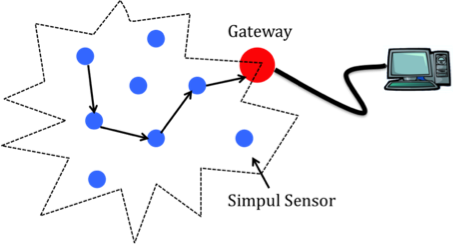
\includegraphics{image/wsn}
          \caption{Jaringan sensor nirkabel.}
          \label{fig:wsn}
      \end{figure}


  \subsection{Sublime Text}
    Et affert civibus has. Has ne facer accumsan argumentum, apeirian hendrerit persequeris pro ex. Suscipit vivendum sensibus mea at, vim ei hinc numquam, at dicit timeam dissentiet mel. At patrioque intellegebat sea, error argumentum dissentias sea in.

    Quo no atqui omnesque intellegat, ne nominavi argumentum quo. Eum ei purto oporteat dissentiet, soleat utamur an sit. Et assum dicam interpretaris quo. Cetero alterum ea vel, no possit alterum utroque nec. His fuisset quaestio ad. Has eu tritani incorrupte consequuntur, esse aliquip nec ne.

% Baris ini digunakan untuk membantu dalam melakukan sitasi
% Karena diapit dengan comment, maka baris ini akan diabaikan
% oleh compiler LaTeX.
\begin{comment}
\bibliography{collection}
\end{comment}


%!TEX root = ./template-skripsi.tex
%-------------------------------------------------------------------------------
%                            BAB III
%               		METODE PENELITIAN
%-------------------------------------------------------------------------------

\chapter{METODE PENELITIAN}

\section{Alat dan Bahan}
	Alat dan bahan yang digunakan pada penelitian ini terbagi atas perangkat keras dan perangkat lunak yang akan dijelaskan seperti berikut.

	\subsection{Perangkat Keras}
		Pro omnium incorrupte ea. Elitr eirmod ei qui, ex partem causae disputationi nec. Amet dicant no vis, eum modo omnes quaeque ad, antiopam evertitur reprehendunt pro ut. Nulla inermis est ne. Choro insolens mel ne, eos labitur nusquam eu, nec deserunt reformidans ut. His etiam copiosae principes te, sit brute atqui definiebas id.

		\vspace{-0.5cm}

		\begin{enumerate}
		\begin{singlespace}
		\itemsep0em
			\item Kit pancar-rima IQRF TR-53B (3 unit),
			\item Kit pengunduh program CK-USB-04 (1 unit),
			\item Kit pengembangan DK-EVAL-03 (2 unit),
			\item Kit pengembangan CK-EVAL-04 (1 unit),
			\item \emph{XBee 802.15.4 Radios (Series 1)} (3 unit),
			\item \emph{XBee Explorer USB Board} (1 unit),
			\item \emph{2 channel Relay Shield For Arduino (With XBee/BTBee interface)} (2 unit),
			\item Arduino Uno (2 unit),
			\item TP-LINK MR3020 (1 unit),
			\item Kabel USB ke Serial Prolific (1 unit).
		\end{singlespace}
		\end{enumerate}

	\subsection{Perangkat Lunak}
		Pro omnium incorrupte ea. Elitr eirmod ei qui, ex partem causae disputationi nec. Amet dicant no vis, eum modo omnes quaeque ad, antiopam evertitur reprehendunt pro ut. Nulla inermis est ne. Choro insolens mel ne, eos labitur nusquam eu, nec deserunt reformidans ut. His etiam copiosae principes te, sit brute atqui definiebas id.

		\vspace{-0.5cm}

		\begin{enumerate}
		\begin{singlespace}
		\itemsep0em
			\item Arduino for Mac OS X,
			\item CoolTerm,
			\item Driver FTDI for Mac OS X,
			\item PHP, MySQL, dan uHTTPd,
			\item Python dan pustaka PySerial,
			\item IQRF IDE v 2.08 for TR-53B,
			\item SSHFS,
			\item Sublime Text 3.
		\end{singlespace}
		\end{enumerate}

\section{Alur Penelitian}
	Consul graeco signiferumque qui id, usu eu summo dicunt voluptatum, nec ne simul perpetua posidonium. Eos ea saepe prodesset signiferumque. No dolore possit est. Mei no justo intellegebat definitiones, vis ferri lorem eripuit ad. Solum tritani scribentur duo ei, his an adipisci intellegat.

\section{Tahapan Pelaksanaan}
	Consul graeco signiferumque qui id, usu eu summo dicunt voluptatum, nec ne simul perpetua posidonium. Eos ea saepe prodesset signiferumque. No dolore possit est. Mei no justo intellegebat definitiones, vis ferri lorem eripuit ad. Solum tritani scribentur duo ei, his an adipisci intellegat.

\section{Jadwal Kegiatan}
	Quo no atqui omnesque intellegat, ne nominavi argumentum quo. Eum ei purto oporteat dissentiet, soleat utamur an sit. Et assum dicam interpretaris quo. Cetero alterum ea vel, no possit alterum utroque nec. His fuisset quaestio ad. Has eu tritani incorrupte consequuntur, esse aliquip nec ne \ref{jadwal}.

	% Please remember to add \use{multirow} to your document preamble in order to suppor multirow cells
		\begin{table}[H]
		\centering
		\caption{Jadwal Penelitian.}
		\label{jadwal}
		\begin{tabular}{|c|l|l|l|l|l|l|l|}
		\hline
		\multirow{2}{*}{No} & \multirow{2}{*}{Keterangan} & \multicolumn{6}{c|}{Bulan}                                                                                                                          \\ \cline{3-8} 
		                    &                             & 1 & 2 & 3 & 4 & 5 & 6 \\ \hline
		1                   & Studi literatur                                  &\cellcolor{gray} &\cellcolor{gray}&                        &                        &                        &                         \\ \hline
		2                   & Desain                                           &                        &\cellcolor{gray}&\cellcolor{gray}&                        &                        &                         \\ \hline
		3                   & Pembelian bahan                                  &                        &                        &\cellcolor{gray}&                        &                        &                         \\ \hline
		4                   & Pembuatan prototipe                              &                        &                        &\cellcolor{gray}&\cellcolor{gray}&\cellcolor{gray}&                         \\ \hline
		5                   & Uji coba dan perbaikan                           &                        &                        &                        &\cellcolor{gray}&\cellcolor{gray}&                         \\ \hline
		6                   & Penulisan skripsi                                &                        &                        &                        &                        &                        &\cellcolor{gray}\\ \hline
		\end{tabular}
		\end{table}
	
% Baris ini digunakan untuk membantu dalam melakukan sitasi
% Karena diapit dengan comment, maka baris ini akan diabaikan
% oleh compiler LaTeX.
\begin{comment}
\bibliography{daftar-pustaka}
\end{comment}


%!TEX root = ./template-skripsi.tex
%-------------------------------------------------------------------------------
%                            BAB IV
%               		HASIL DAN PEMBAHASAN
%-------------------------------------------------------------------------------

\chapter{HASIL DAN PEMBAHASAN}
	\section{Subbab 1}
		Habeo perfecto in sea. Ea deleniti gloriatur pri, paulo mediocrem incorrupte sea ei. Ad mollis scripta per. Incorrupte sadipscing ne mel. Mel ex nonumy malorum epicurei.

		Ne per tota mollis suscipit. Ullum labitur vim ut, ea dicit eleifend dissentias sit. Duis praesent expetenda ne sed. Sit et labitur albucius elaboraret. Ceteros efficiantur mei ad. Hendrerit vulputate democritum est at, quem veniam ne has, mea te malis ignota volumus.

		Eros reprimique vim no. Alii legendos volutpat in sed, sit enim nemore labores no. No odio decore causae has. Vim te falli libris neglegentur, eam in tempor delectus dignissim, nam hinc dictas an.
	
	\section{Subbab 2}		
		Habeo perfecto in sea. Ea deleniti gloriatur pri, paulo mediocrem incorrupte sea ei. Ad mollis scripta per. Incorrupte sadipscing ne mel. Mel ex nonumy malorum epicurei.

		\subsection{Subsubbab 2 1}
			Ne per tota mollis suscipit. Ullum labitur vim ut, ea dicit eleifend dissentias sit. Duis praesent expetenda ne sed. Sit et labitur albucius elaboraret. Ceteros efficiantur mei ad. Hendrerit vulputate democritum est at, quem veniam ne has, mea te malis ignota volumus.
			
			\begingroup
			    \fontsize{10pt}{12pt}\selectfont
			    \begin{verbatim}
					config mount
				        option target        /mnt
				        option device        /dev/sda1
				        option fstype        ext3
				        option options       rw,sync
				        option enabled       1
				        option enabled_fsck  0
				        option is_rootfs     1
			    \end{verbatim}  
			\endgroup

			\begingroup
			    \fontsize{10pt}{12pt}\selectfont
			    \begin{verbatim}
					# opkg update
					# opkg install python pyserial
			    \end{verbatim}  
			\endgroup			

		\subsection{Subsubbab 2 2}
			Consul graeco signiferumque qui id, usu eu summo dicunt voluptatum, nec ne simul perpetua posidonium. Eos ea saepe prodesset signiferumque. No dolore possit est. Mei no justo intellegebat definitiones, vis ferri lorem eripuit ad. Solum tritani scribentur duo ei, his an adipisci intellegat.

	\section{Subab 3}
		Consul graeco signiferumque qui id, usu eu summo dicunt voluptatum, nec ne simul perpetua posidonium. Eos ea saepe prodesset signiferumque. No dolore possit est. Mei no justo intellegebat definitiones, vis ferri lorem eripuit ad. Solum tritani scribentur duo ei, his an adipisci intellegat.
			
			
% Baris ini digunakan untuk membantu dalam melakukan sitasi.
% Karena diapit dengan comment, maka baris ini akan diabaikan
% oleh compiler LaTeX.
\begin{comment}
\bibliography{collection}
\end{comment}

%!TEX root = ./template-skripsi.tex
%-------------------------------------------------------------------------------
%                            	BAB V
%               			PENUTUP
%-------------------------------------------------------------------------------

 \chapter{PENUTUP}

\section{Kesimpulan}
	Berdasarkan hasil analisis dan pengujian fungsional aplikasi ini, didapat kesimpulan sebagai berikut \citep[12-17]{Bhanot2015}

	\begin{enumerate}
		\item Lorem ipsum is a pseudo-Latin text used in web design, typography, layout, and printing in place of English to emphasise design elements over content. 
		
		\item It's also called placeholder (or filler) text. It's a convenient tool for mock-ups. 
		
		\item It helps to outline the visual elements of a document or presentation, eg typography, font, or layout. Lorem ipsum is mostly a part of a Latin text by the classical author and philospher Cicero.

		\item Its words and letters have been changed by addition or removal, so to deliberately render its content nonsensical; it's not genuine, correct, or comprehensible Latin anymore \citet[30-35]{Cui2014}. 
	\end{enumerate}


\section{Saran}
	\begin{enumerate}
		\item Lorem ipsum is a pseudo-Latin text used in web design, typography, layout, and printing in place of English to emphasise design elements over content. 
		
		\item It's also called placeholder (or filler) text. It's a convenient tool for mock-ups. 
		
		\item It helps to outline the visual elements of a document or presentation, eg typography, font, or layout. Lorem ipsum is mostly a part of a Latin text by the classical author and philospher Cicero.

		\item Its words and letters have been changed by addition or removal, so to deliberately render its content nonsensical; it's not genuine, correct, or comprehensible Latin anymore. 
	\end{enumerate}

	
% Baris ini digunakan untuk membantu dalam melakukan sitasi
% Karena diapit dengan comment, maka baris ini akan diabaikan
% oleh compiler LaTeX.

\begin{comment}
\bibliography{collection}
\end{comment}


%-----------------------------------------------------------------
%Disini akhir masukan Bab
%-----------------------------------------------------------------


%-----------------------------------------------------------------
% Disini awal masukan untuk Daftar Pustaka
% - Daftar pustaka diambil dari file .bib yang ada pada folder ini
%   juga.
% - Untuk memudahkan dalam memanajemen dan menggenerate file .bib
%   gunakan reference manager seperti Mendeley, Zotero, EndNote,
%   dll.
%-----------------------------------------------------------------

\bibliography{collection}
\addcontentsline{toc}{chapter}{DAFTAR PUSTAKA}

%-----------------------------------------------------------------
%Disini akhir masukan Daftar Pustaka
%-----------------------------------------------------------------

%!TEX root = ./template-skripsi.tex
%-------------------------------------------------------------------------------
%               		LAMPIRAN
%-------------------------------------------------------------------------------

\addcontentsline{toc}{chapter}{LAMPIRAN}
  \chapter*{LAMPIRAN}%

\appendix
\newappendix{Lampiran 1}
Lorem ipsum is a pseudo-Latin text used in web design, typography, layout, and printing in place of English to emphasise design elements over content. 
		
\newappendix{Lampiran 3} 
 It's also called placeholder (or filler) text. It's a convenient tool for mock-ups. 
		
\newappendix{Lampiran 3} 
 It helps to outline the visual elements of a document or presentation, eg typography, font, or layout. Lorem ipsum is mostly a part of a Latin text by the classical author and philospher Cicero.

\newappendix{Lampiran 4}
Its words and letters have been changed by addition or removal, so to deliberately render its content nonsensical; it's not genuine, correct, or comprehensible Latin anymore



	\begin{enumerate}
		\item Lorem ipsum is a pseudo-Latin text used in web design, typography, layout, and printing in place of English to emphasise design elements over content. 
		
		\item It's also called placeholder (or filler) text. It's a convenient tool for mock-ups. 
		
		\item It helps to outline the visual elements of a document or presentation, eg typography, font, or layout. Lorem ipsum is mostly a part of a Latin text by the classical author and philospher Cicero.

		\item Its words and letters have been changed by addition or removal, so to deliberately render its content nonsensical; it's not genuine, correct, or comprehensible Latin anymore. 
	\end{enumerate}

	



\end{document}

